%!TEX root = /Users/simo/Documents/PFC/Chapter3/chapter3.tex
\section{Sexto Ciclo} % (fold)
\label{sec:sexto_ciclo}

La siguiente iteración intentará solucionar un problema aparecido en el ciclo anterior, y requiere de un enfoque distinto para el proceso de generación de páginas en masa a partir de PDF's o archivos comprimidos. Pero previa comprensión de las razones por las que puede haber un problema en este proceso, es necesario entender como funcionaría una web funcionando en Ruby on Rails en un entorno \emph{real}.

La forma de mantener un servidor web sirviendo una aplicación desarrollada en Ruby on Rails, es teniendo una o varias instancias de dicha aplicación sirviendo páginas. Cada instancia de dicha aplicación puede servir solamente una página a la vez, pero puesto que están cargadas todas las librerías, y además se utilizan múltiples técnicas de cacheo, y que por tanto no es necesario recargar código después de cada consulta, dichas páginas se sirven de forma extremadamente rápida.

Esto, sin embargo, quiere decir que mientras una aplicación está ocupada sirviendo una petición, no puede atender a otra. Generalmente, páginas normales de la aplicación tienen un tiempo de generación minúsculo, pero ante tareas como las que atañen a este ciclo (conversión de PDF's y descompresión de archivos), significan mantener una de dichas instancias ocupadas durante segundos enteros. Así, por tanto, en cuanto hubiera una cantidad de personas subiendo archivos igual a la cantidad de instancias del servidor, nadie podría navegar, pues todas las instancias estarían ocupadas. No solo eso, sino que tener varios procesos realizando operaciones de actividad intesiva de CPU, y que además suelen necesitar de memoria extra, no es una situación deseable.

Éste es un problema similar al que afrontan servicios similares, como podrían ser, por ejemplo, cualquiera de los servicio de subida de vídeos como Youtube o Vimeo, y la solución para estos problemas, es la de tener un proceso a parte dedicado solamente a realizar dichas tareas. Este proceso, al ser solamente uno, evita situaciones en que el sistema pueda estar saturado tanto por no quedar instancias disponibles a los usuarios para seguir visitando la web, como por tener múltiples procesos intensivos de CPU realizándose al mismo tiempo.

\subsection{Análisis de requisitos} % (fold)
\label{sub:análisis_de_requisitos}

\begin{itemize}
  \item Implementar un mecanismo de forma que pueda existir un proceso a parte dedicado a realizar tareas costosas.
  \item Que el código actual utilice dicho sistema.
\end{itemize}

% subsection análisis_de_requisitos (end)

\subsection{Diseño} % (fold)
\label{sub:diseño}

La dinámica de funcionamiento para esta nueva funcionalidad, será la de ir creando tareas que el proceso aparté irá procesando. Es necesario pues, almacenar dichas tareas en la base de datos, con los datos necesarios para poder ser recuperadas y procesadas a posteriori. Este nuevo modelo, al que se llamará \texttt{Task}, aparece en el diagrama de clases de la siguiente forma:

\begin{figure}[h!]
\centering
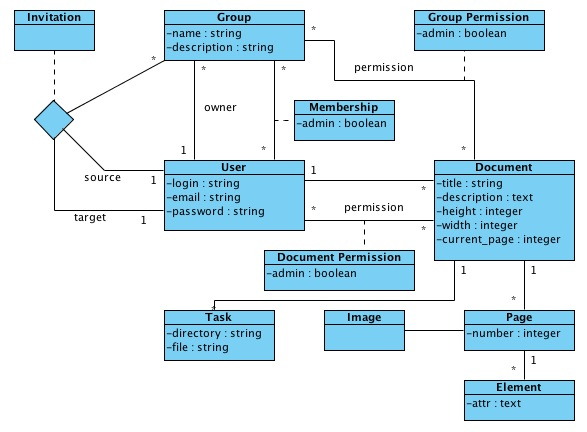
\includegraphics[width=14cm]{uml6.png}
\caption{Clases del dominio, 6º ciclo}\label{fig:uml6}
\end{figure}

% subsection diseño (end)

\subsection{Implementación} % (fold)
\label{sub:implementación}

Este problema, como ya se ha comentado, es muy común en este tipo de servicios, con lo que existe un plugin adecuado, mucho más completo que si esta parte del código se hubiera tenido que programar desde cero. Dicho plugin es \texttt{delayed\_jobs} \footnote{http://github.com/tobi/delayed\_job} , fruto del trabajo de la web Shopify \footnote{http://www.shopify.com/}, un servicio de hosting de e-commerce, y que ha publicado su sistema de ejecución de tareas de forma pública en modo de plugin.

Este plugin generaliza mucho más de lo que se había pensado inicialmente, y es capaz de almacenar cualquier tipo de modelo, serializándolo para posterior recuperación, ejecutando siempre la función \texttt{perform}, de forma que con un solo proceso es posible realizar cualquier tipo de tarea que se quiera \emph{separar} del flujo normal de trabajo. En este caso no es necesario, pero es perfectamente adecuado para posibles necesidades en el futuro.

La forma en que funciona es teniendo una tabla propia de tareas, llamadas \texttt{Jobs}, de forma que, en realidad, harían falta dos nuevos modelos para poder desepeñar estos trabajos, pero puesto que el plugin se encarga de almacenar el objeto que debe procesar serializándolo, es posible implementar un modelo que no tenga porqué estar reflejado en la base de datos.

La forma en que Rails hace que un modelo esté automáticamente replicado en la base de datos es mediante el motor \texttt{ActiveRecord}. Si en vez de heredar el modelo Task de ActiveRecord, se hereda de un objeto más simple, como un Struct, se tiene un modelo personalizable, que \texttt{delayed\_jobs} puede serializar de forma muy sencilla, y que puede tener implementadas igualmente funciones. Así pues, la clase Task quedaría así:
\begin{verbatim}
class Task < Struct.new(:document_id, :directory, :file)
  def perform
    # procesar el archivo file que está en el directorio directory,
    # y asignar las páginas generadas al documento document_id
  end    
end
\end{verbatim}

Y a la hora de añadir una \texttt{Task} a la cola de tareas de \texttt{delayed\_jobs}:

\begin{verbatim}
  Delayed::Job.enqueue Task.new(document,directory,file)
\end{verbatim}

Para ejecutar el proceso que se encarta de ir reclamando \texttt{Jobs} e ir ejecutando sus funciones \texttt{perform}:

\begin{verbatim}
  $ rake jobs:work
\end{verbatim}

Este proceso no se parará aunque las funciones que se ejecuten salten una excepción, sinó que la capturará y guardará el mensaje de error para posterior revision, evitando así que tareas defectuosas o maliciosas puedan perjudicar al resto de elementos a procesar.

% subsection implementación (end)

% section cuarto_ciclo (end)